\section{Filtros Continuos}
\subsection{Filtros continuos generales}


\begin{frame}
    \frametitle{Filtros Continuos Generales I}
    \footnotesize
    El comportamiento en frecuencia de un filtro continuo queda determinado por la posici\'{o}n de los polos y los ceros de su funci\'{o}n de transferencia $H(s)$.
    \vspace{0.1cm}
    Podemos recordar, de sistemas lineales, los comportamientos que se observan al representar la respuesta en frecuencia de diferentes filtros b\'{a}sicos (sistemas estables).
    \vspace{0.1cm}

    \begin{columns}[c]
        \hspace{0.7cm}\begin{column}{6cm}
            \alert{Polo simple}: $H(s)=\frac{a}{s+a}$, (\color{olivegreen}Ej: \color{black}a=10)
            \vspace{0.1cm}
            \scriptsize
            Atenúa, pero no totalmente.
            Si usamos varios polos simples atenuará  mas rápido.
            \vspace{0.1cm}
            \begin{figure}\centering
                \includegraphics[width=5cm]{./Figures/FiltroContinuo1b.eps}
            \end{figure}
            \vspace{-0.4cm}
        \end{column}

        \begin{column}{6cm}
            \vspace{-0.0cm}
            \alert{Cero simple: }$H(s)=\frac{s+a}{a}$, (\color{olivegreen}Ej: \color{black}a=10)
            \vspace{0.2cm}\scriptsize
            Amplifica, continuamente.
            \vspace{0.1cm}
            \begin{figure}\centering
                \includegraphics[width=5cm]{./Figures/FiltroContinuo2b.eps}
            \end{figure}
        \end{column}
    \end{columns}
\end{frame}


\begin{frame}
    \frametitle{Filtros Continuos Generales II}

    \footnotesize
    \begin{columns}[c]
        \hspace{0.7cm}\begin{column}{6cm}
            \alert{Polo doble: }$H(s)=\frac{\sigma^2+\omega_a^2}{s^2+2\sigma s +\sigma^2+\omega_a^2 }$,
            \scriptsize
            \vspace{0.1cm}
            \hspace{1.6cm}(\color{olivegreen}Ej: \color{black} $\sigma=1$, $\omega_a=3$)
            \vspace{-0.1cm}
            \begin{figure}\centering
                \includegraphics[width=3.5cm]{./Figures/FiltroContinuo3b.eps}
            \end{figure}
        \end{column}
        \begin{column}{6cm}
            \alert{Cero doble: }$H(s)=\frac{s^2+2\sigma s +\sigma^2+w_a^2 }{\sigma^2+w_a^2}$,
            \scriptsize
            \vspace{0.1cm}
            \hspace{1.6cm}(\color{olivegreen}Ej: \color{black} $\sigma=1$, $w_a=3$)
            \vspace{-0.1cm}
            \visible<2->{\begin{figure} \centering \includegraphics[width=3.5cm]{./Figures/FiltroContinuo4b.eps}  \end{figure}}
        \end{column}
    \end{columns}

    \begin{columns}[c]
        \hspace{0.7cm}\begin{column}{6cm}
        \alert{Polo doble:}$H(s)=\frac{\omega_n^2}{s^2+\omega_n^2 }$,  (\color{olivegreen}Ej: \color{black} $\omega_n=3$)
        \scriptsize
        \vspace{0.1cm}
        Es inestable para $\omega=\omega_n$
        \vspace{-0.1cm}
        \begin{figure}\centering
            \includegraphics[width=3.5cm]{./Figures/FiltroContinuo5b.eps}
        \end{figure}
    \end{column}
    \vspace{0.1cm}
    \begin{column}{6cm}
        \alert{Cero doble: }$H(s)=\frac{s^2+\omega_n^2 }{\omega_n^2}$, (\color{olivegreen}Ej: \color{black}$\omega_n=3$)
        \scriptsize
        \vspace{0.1cm}
        atenua totalmente a $\omega=\omega_n$
        \vspace{-0.1cm}
        \begin{figure}\centering
            \includegraphics[width=3.5cm]{./Figures/FiltroContinuo6b.eps}
        \end{figure}
        \end{column}
    \end{columns}
\end{frame}

%%%%%%%%%%%%%%%%%%%%%%%%%%%%%


\begin{frame}
    \frametitle{Filtros Continuos Generales III}
    \footnotesize
    Para obtener la función de transferencia de un filtro continuo podemos:
    \begin{itemize}
        \item Colocar dos ceros imaginarios puros sobre las frecuencias $\omega_n$ que deseamos eliminar completamente
        \item Compensar la amplificación asociada a cada cero, con un polo con parte real negativa (eligiendo el valor de la $a$ o de la $\omega_a$ de forma apropiada).
        \item Necesitamos al menos tantos polos como ceros que el sistema sea causal (y para atenuar la amplificación continua final asociada a cada cero).
    \end{itemize}
    Sin embargo, este método no es siempre trivial (muchos parámetros).
\end{frame}
